
\begin{resumeBox}
  \emph{À retenir dans une semaine :} 
  \begin{niceitemize}
    \item Nous interprèterons les vecteurs plutôt comme des points, et pas comme des flèches.
    \item Pour résoudre un système linéaire, on le rend \textbf{échelonné} avec le pivot de Gauss.
    \item On peut interpréter un système linéaire de 3 façons différentes : 
      \begin{itemize}
        \item[$\bullet$] Comme une intersection d'éléments géométriques (droites, plans, etc.).
        \item[$\bullet$] Comme une combinaison linéaire de vecteurs.
        \item[$\bullet$] Comme une équation matricielle.
      \end{itemize}
  \end{niceitemize}
\end{resumeBox}
% \begin{formulesBox}
%   % Placez ici vos formules, figures TikZ ou images.
%   % Exemple : $F(\omega)=\int_{-\infty}^{+\infty} f(t)\,e^{-i\omega t}\,dt$
%   % \begin{center}\includegraphics[width=.8\linewidth]{exemple.jpg}\end{center}
% \end{formulesBox}
\begin{rappelsBox}
  \begin{niceitemize}
    \item Que signifie qu'un système soit échelonné ?
    \item Quelles sont les manipulations autorisées pour le pivot de Gauss ?
    \item Comment interpréter un système linéaire comme une combinaison de vecteurs ?
  \end{niceitemize}
\end{rappelsBox}

\section{Exercices}
  \subsection{Équations de réactions chimiques}
  Les équations de réactions chimiques peuvent être interprétées comme des systèmes linéaires. \newline
  Y a-t-il toujours une infinité de façon d'équilibrer l'équation ?


  \vspace{1em}

  Transformer le problème suivant en système linéaire. Sans le résoudre, combien a-t-il de solutions ?
  \begin{center}
    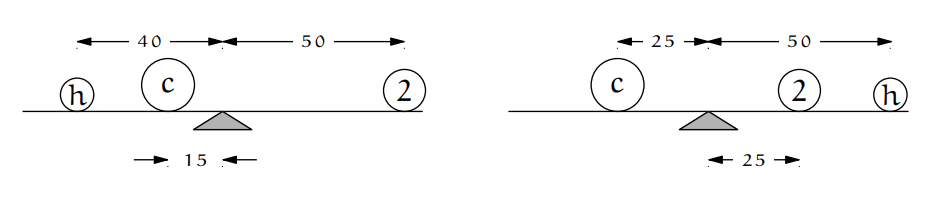
\includegraphics[width=0.8\linewidth]{0-Revisions/2-PivotDeGauss/equilibre.png}
  \end{center}

  \newpage

  \vspace{2em}

  \subsection{Combien de solutions ?}
Ces systèmes admettent-ils zéro, une ou une infinité de solutions ?

% Correction (affichée seulement si showSolutions=true)
\ifthenelse{\boolean{showSolutions}}{%
\textbf{Correction}
\begin{multicols}{3}
\begin{enumerate}[label=\alph*)]
\item une solution unique
\item une infinité de solutions
\item une infinité de solutions
\item aucune solution
\item une infinité de solutions
\item une infinité de solutions
\item aucune solution
\item une infinité de solutions
\item aucune solution
\item une solution unique
\end{enumerate}
\end{multicols}
}{}

\begin{multicols}{3}
\begin{enumerate}[label=\alph*)]
\item $$\begin{cases}
    -3x + 2y &= 0\\
    -2y &= 0
  \end{cases}$$

\item $$\begin{cases}
    x + y &= 4\\
    y - z &= 0
  \end{cases}$$

\item 
$$\begin{cases}
    x + y &= 4\\
    y - z &= 0\\
    0 &= 0
  \end{cases}$$

\item 
$$\begin{cases}
    x + y &= 4\\
    0 &= 4
  \end{cases}$$

\item 
$$\begin{cases}
    3x + 6y + z &= -0.5\\
    -z &= 2.5
  \end{cases}$$

\item 
$$\begin{cases}
    x - 3y &= 2\\
    0 &= 0
  \end{cases}$$

\item 
$$\begin{cases}
    2x + 2y &= 4\\
    y &= 1\\
    0 &= 4
  \end{cases}$$

\item 
$$\begin{cases}
    2x + y &= 0
  \end{cases}$$

\item 
$$\begin{cases}
    x - y &= -1\\
    0 &= 0\\
    0 &= 4
  \end{cases}$$

\item 
$$\begin{cases}
    x + y - 3z &= -1\\
    y - z &= 2\\
    z &= 0\\
    0 &= 0
  \end{cases}$$
\end{enumerate}
\end{multicols}



\vspace{2em}
\subsection{Systèmes d'équations linéaires}
Résoudre les systèmes suivants :

% Correction (affichée seulement si showSolutions=true)
\ifthenelse{\boolean{showSolutions}}{%
\textbf{Correction}
\begin{multicols}{3}
\begin{enumerate}[label={}]
\item $(x,y) = \left(2,\tfrac{1}{2}\right)$
\item $(x,y) = \left(\tfrac{1}{2},\tfrac{3}{2}\right)$
\item $\{(x,y,z)=(-12+7t,\ t,\ 13-4t),\ t\in\mathbb{R}\}$
\item aucune solution
\item $(x,y,z)=(5,5,0)$
\item $\{(x,y,z,w)=(1,\ t-1,\ 3-t,\ t),\ t\in\mathbb{R}\}$
\end{enumerate}
\end{multicols}
}{}

\begin{multicols}{3}
\begin{enumerate}[label={}]
\item 
$$\begin{cases}
  2x + 2y = 5 \\
    x - 4y = 0
  \end{cases}$$

\item 
  $$\begin{cases}
    -x + y = 1 \\
    x + y = 2
  \end{cases}$$

\item 
$$\begin{cases}
    x - 3y + z = 1 \\
    x + y + 2z = 14
  \end{cases}$$


\item 
$$\begin{cases}
    -x - y = 1 \\
    -3x - 3y = 2
  \end{cases}$$


\item 
$$\begin{cases}
    4y + z = 20 \\
    2x - 2y + z = 0 \\
    x + z = 5 \\
    x + y - z = 10
  \end{cases}$$


\item 
$$\begin{cases}
    2x + z + w = 5 \\
    y - w = -1 \\
    3x - z - w = 0 \\
    4x + y + 2z + w = 9
  \end{cases}$$

\end{enumerate}
\end{multicols}

\vspace{2em}

\subsection{Approfondissement}
Résoudre 
$$\begin{cases}
  2 \sin \alpha-\cos \beta+3 \tan \gamma &= 3 \\
  4 \sin \alpha+2 \cos \beta-2 \tan \gamma &= 10 \\
  6 \sin \alpha-3 \cos \beta+\tan \gamma &= 9
\end{cases}$$

% Correction (affichée seulement si showSolutions=true)
\ifthenelse{\boolean{showSolutions}}{%
\medskip
En posant $u=\sin\alpha$, $v=\cos\beta$, $w=\tan\gamma$, on obtient le système linéaire
\[\begin{cases}
2u-v+3w=3,\\
2u+v-w=5,\\
6u-3v+w=9.
\end{cases}\]
Sa solution est $(u,v,w)=(2,1,0)$. Comme $\sin\alpha\in[-1,1]$, ceci est impossible, donc \textbf{pas de solution réelle}.
}{}

\newpage
\vspace{2em}

\subsection{Manipulation}

\textit{La méthode de Gauss consiste à combiner les équations d'un système pour en former de nouvelles.}

\medskip
\begin{enumerate}[label=\alph*)]
\item Peut-on obtenir l'équation \(3x - 2y = 5\) par une suite d'opérations de réduction de Gauss à partir des équations de ce système ?
\[
\begin{cases}
x + y = 1 \\
4x - y = 6
\end{cases}
\]

\item Peut-on obtenir l'équation \(5x - 3y = 2\) par une suite d'opérations de réduction de Gauss à partir des équations de ce système ?
\[
\begin{cases}
2x + 2y = 5 \\
3x + y = 4
\end{cases}
\]

\item Peut-on obtenir \(6x - 9y + 5z = -2\) par une suite d'opérations de réduction de Gauss à partir des équations de ce système ?
\[
\begin{cases}
2x + y - z = 4 \\
6x - 3y + z = 5
\end{cases}
\]
\end{enumerate}

% Correction (affichée seulement si showSolutions=true)
\ifthenelse{\boolean{showSolutions}}{%
\medskip
\textbf{Correction}
\begin{enumerate}[label=\alph*)]
\item Oui. $-E_1+E_2$ donne $3x-2y=5$.
\item Non. Aucune combinaison linéaire des équations ne peut donner un second membre égal à $2$.
\item Oui. $-3E_1+2E_2$ donne $6x-9y+5z=-2$.
\end{enumerate}
}{}

\vspace{2em}
\subsection{Interprétation}
Choisir 3 systèmes linéaire dans un exercice précédent et l'écrire des 2 manières différentes : 
\begin{enumerate}
\item Comme une combinaison linéaires de vecteurs.
\item Comme une équation matricielle.
\end{enumerate}

Par exemple, le système 
$$\begin{cases}
x + y = 1 \\
4x - y = 6
\end{cases}$$
peut s'écrire comme une combinaison linéaire de vecteurs :
$$x\begin{pmatrix}1\\4\end{pmatrix} + y\begin{pmatrix}1\\-1\end{pmatrix} = \begin{pmatrix}1\\6\end{pmatrix}$$
ou comme une équation matricielle :
$$\begin{pmatrix}1&1\\4&-1\end{pmatrix}\begin{pmatrix}x\\y\end{pmatrix} = \begin{pmatrix}1\\6\end{pmatrix}$$

\vspace{2em}
\subsection{Pour ceux qui s'ennuient}
Une boîte contenant des pennies, des nickels et des dimes renferme treize pièces d'une valeur totale de 83 cents.
Combien y a-t-il de pièces de chaque type dans la boîte ?
(Ce sont des pièces américaines : un penny vaut 1 cent, un nickel 5 cents et un dime 10 cents.)

% Correction (affichée seulement si showSolutions=true)
\ifthenelse{\boolean{showSolutions}}{%
\medskip
Soient $p,n,d$ le nombre de pennies, nickels, dimes. On a
\[\begin{cases}
p+n+d=13,\\
p+5n+10d=83.
\end{cases}\]
On en déduit $4n+9d=70$, donc $d\equiv2\ (\mathrm{mod}\ 4)$. L'unique solution entière non négative est $d=6$, $n=4$, $p=3$.
}{}
